%% ============================================================================
\begin{frame}[fragile]
\frametitle{CUDA design goals}

\begin{itemize}
\item Enable heterogeneous systems (i.e., CPU+GPU)
\item Scale to 100's of cores, 1000's of parallel threads
\item Use C/C++ with minimal extensions
\item Let programmers focus on parallel algorithms
\end{itemize}

\begin{center}
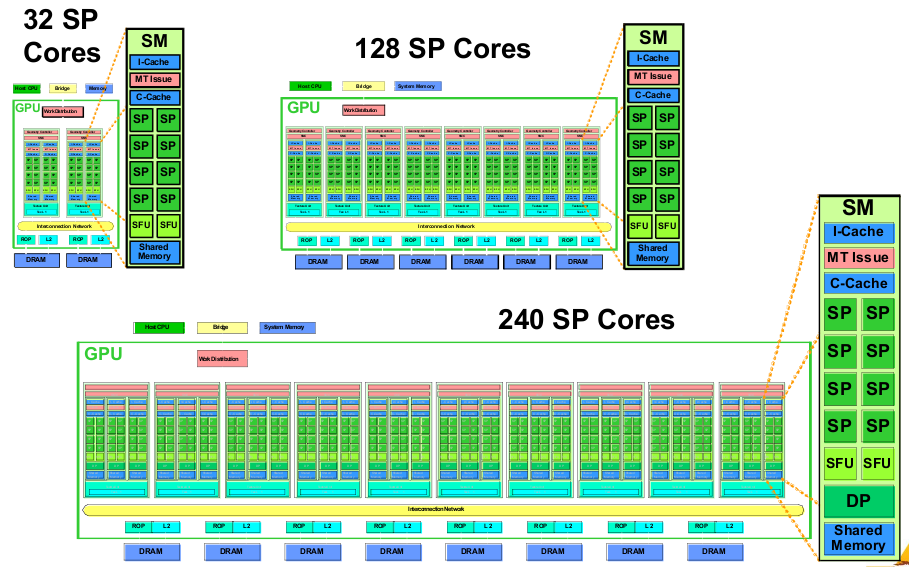
\includegraphics[scale=0.38]{images/1.png}
\end{center}

\end{frame}
%% ============================================================================
%% ============================================================================
\begin{frame}[fragile]
\frametitle{Heterogeneous programming (1/3)}

\begin{itemize}
\item A CUDA program is a serial program with parallel kernels, all in C.
\item The serial C code executes in a \textcolor{blue}{host} (= CPU) thread
\item The parallel kernel C code executes in many \textcolor{blue}{device} 
   threads across multiple GPU processing elements, called 
\textcolor{blue}{streaming processors} (SP).
\end{itemize}

\begin{center}
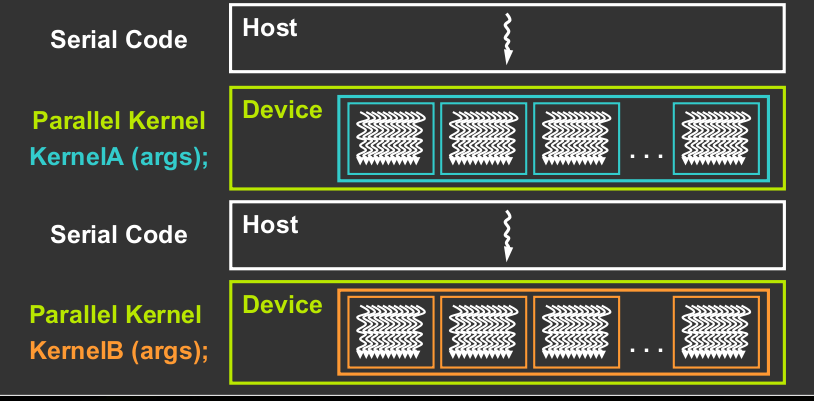
\includegraphics[scale=0.5]{images/Z-17.png}
\end{center}

\end{frame}
%% ============================================================================
%% ============================================================================
\begin{frame}[fragile]
\frametitle{Heterogeneous programming (2/3)}

\begin{itemize}
\item Thus, the parallel code (kernel) is launched and executed on a
      device by many threads.
\item Threads are grouped into thread blocks.
\item One kernel is executed at a time on the device.
\item Many threads execute each kernel.
\end{itemize}

\begin{center}
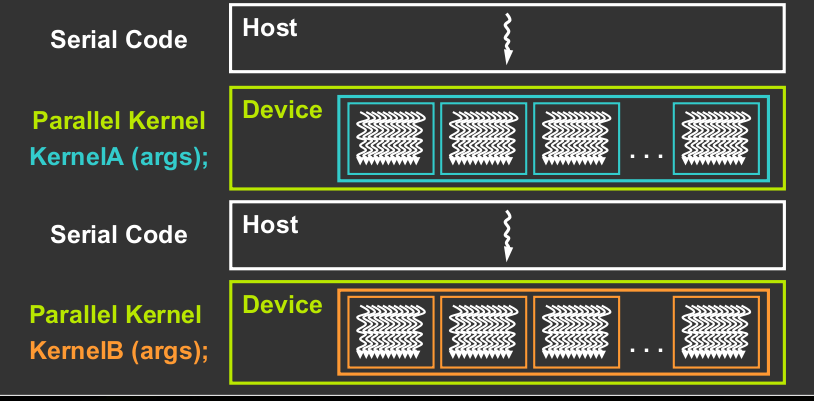
\includegraphics[scale=0.4]{images/Z-17.png}
\end{center}

\end{frame}
%% ============================================================================
%% ============================================================================
\begin{frame}[fragile]
\frametitle{Heterogeneous programming (3/3)}

\begin{itemize}
\item The parallel code is written for a thread
\begin{itemize}
\item Each thread is free to execute a unique code path
\item Built-in \textcolor{blue}{\bf thread and block ID variables}
      are used to map each thread to a specific data tile (see next slide).
\end{itemize}
\item Thus, each thread executes the same code
      on different data based on its thread and block ID.
\end{itemize}

\begin{center}
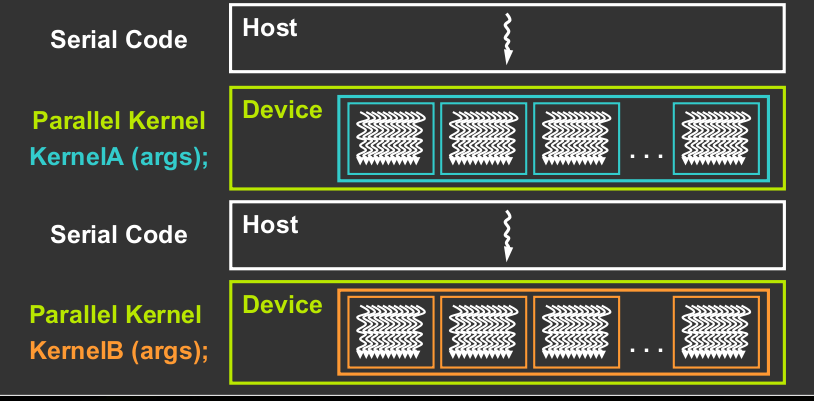
\includegraphics[scale=0.4]{images/Z-17.png}
\end{center}

\end{frame}
%% ============================================================================
%% ============================================================================
\begin{frame}[fragile]
\frametitle{Example: increment array elements (1/2)}

\begin{center}
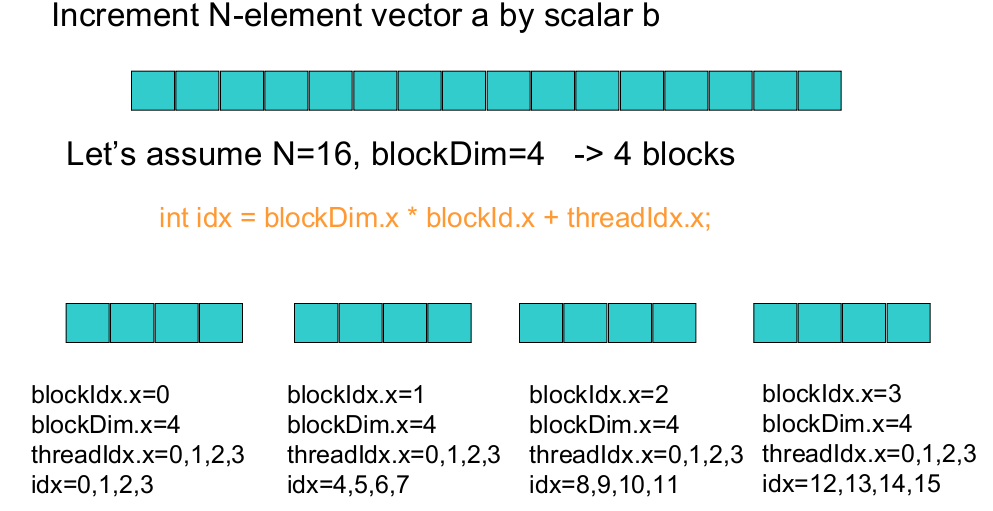
\includegraphics[scale=0.5]{images/7.png}
\end{center}

See our exampe number 4 in {\tt /usr/local/cs4402/examples/4}

\end{frame}
%% ============================================================================
%% ============================================================================
\begin{frame}[fragile]
\frametitle{Example: increment array elements (2/2)}

\begin{center}
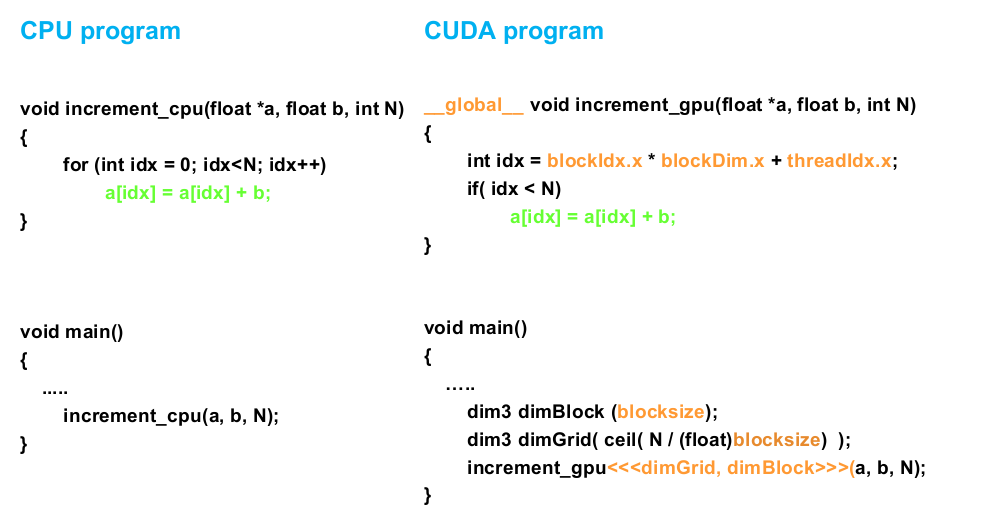
\includegraphics[scale=0.5]{images/8.png}
\end{center}
\end{frame}
%% ============================================================================
%% ============================================================================
\begin{frame}[fragile]
\frametitle{Thread blocks (1/2)}

\begin{itemize}
\item A \textcolor{blue}{\bf Thread block} is a group of threads that can:
\begin{itemize}
\item Synchronize their execution
\item Communicate via shared memory
\end{itemize}
\item Within a grid, \textcolor{red}{\bf thread blocks can run in any order}:
\begin{itemize}
\item  Concurrently or sequentially
\item  Facilitates scaling of the same code across many devices
\end{itemize}
\end{itemize}

\begin{center}
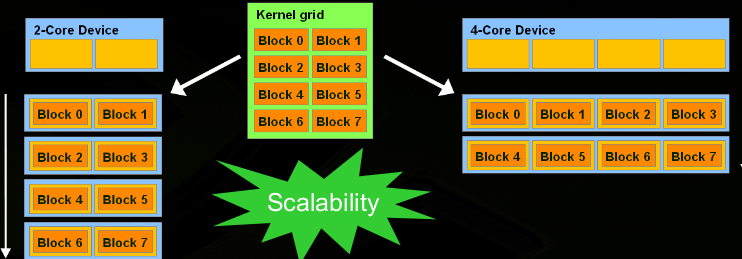
\includegraphics[scale=0.5]{images/11.png}
\end{center}
\end{frame}
%% ============================================================================
%% ============================================================================
\begin{frame}[fragile]
\frametitle{Thread blocks (2/2)}

\begin{itemize}
\item Thus, within a grid, any possible interleaving of 
       blocks must be valid.
\medskip
\item Thread blocks  \textcolor{red}{\bf may coordinate but not synchronize}
\begin{itemize}
\item they may share pointers
\item they should not share locks (this can easily deadlock).
\end{itemize}
\medskip
\item The fact that thread blocks cannot synchronize
     gives \textcolor{blue}{\bf scalability}:
\begin{itemize}
\item A kernel scales across any number of parallel cores
\end{itemize}
\medskip
\item However, within a thread bloc,  
    threads in the same block may synchronize with barriers.
\item That is, threads wait at the barrier until threads 
     in the  \textcolor{red}{\bf same block} reach the barrier.
\end{itemize}

\end{frame}
%% ============================================================================
%% ============================================================================
\begin{frame}[fragile]
\frametitle{Memory hierarchy (1/3)}

\textcolor{blue}{\bf Host (CPU) memory}:
\begin{itemize}
\item Not directly accessible by CUDA threads
\end{itemize}

\begin{center}
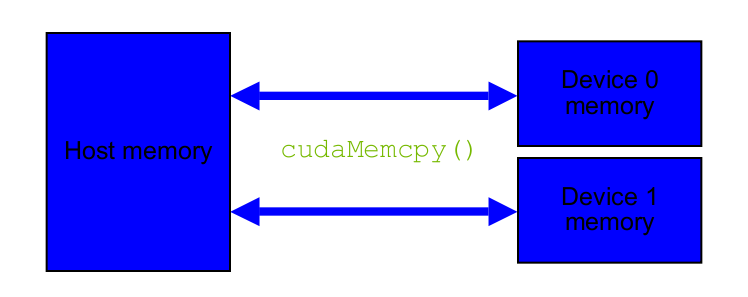
\includegraphics[scale=0.6]{images/15.png}
\end{center}
\end{frame}
%% ============================================================================
%% ============================================================================
\begin{frame}[fragile]
\frametitle{Memory hierarchy (2/3)}

\textcolor{blue}{\bf Global (on the device) memory}:
\begin{itemize}
\item Also called \textcolor{blue}{\bf device memory}
\item Accessible by all threads as well as host (CPU)
\item Data lifetime = from allocation to deallocation
\end{itemize}


\begin{center}
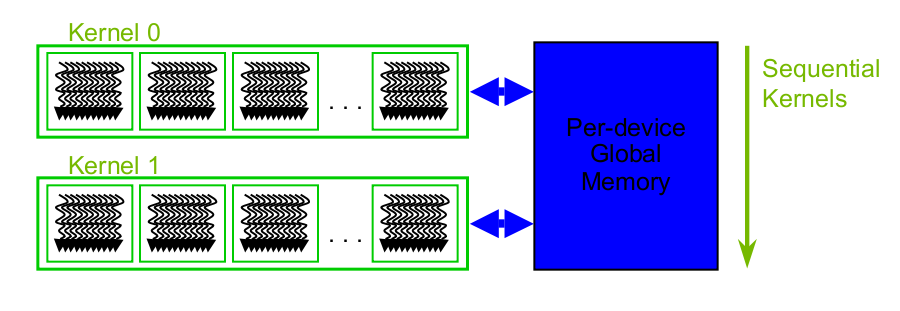
\includegraphics[scale=0.5]{images/14.png}
\end{center}
\end{frame}
%% ============================================================================
%% ============================================================================
\begin{frame}[fragile]
\frametitle{Memory hierarchy (3/3)}

\textcolor{blue}{\bf Shared memory}:
\begin{itemize}
\item  Each thread block has its own shared memory,
       which is accessible only by the threads within that block
\item Data lifetime = block lifetime
\end{itemize}

\textcolor{blue}{\bf Local storage}:
\begin{itemize}
\item Each thread has its own local storage
\item Data lifetime = thread lifetime
\end{itemize}

\begin{center}
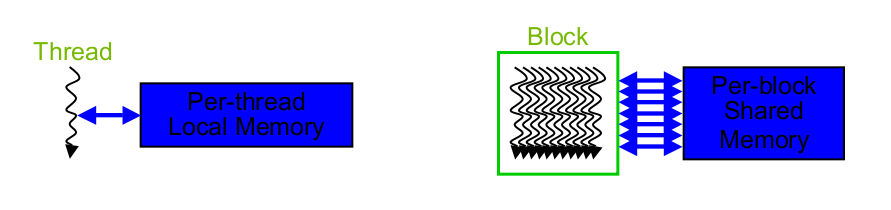
\includegraphics[scale=0.5]{images/13.png}
\end{center}
\end{frame}
%% ============================================================================
%% ============================================================================
\begin{frame}[fragile]
\frametitle{Blocks run on multiprocessors}


\begin{center}
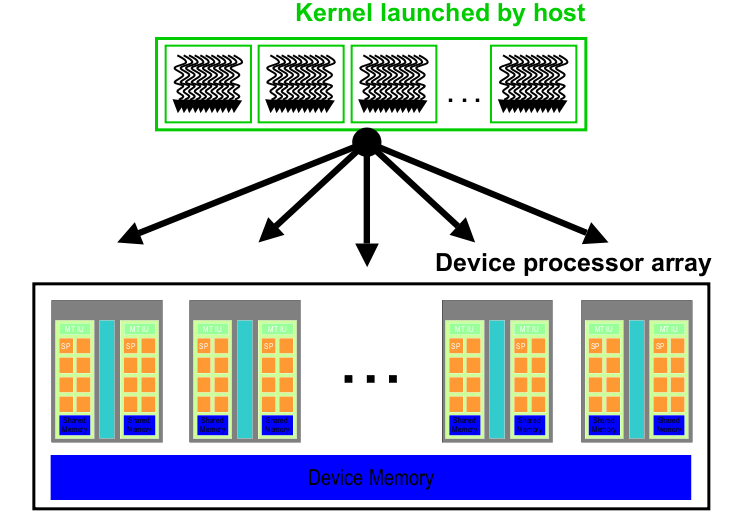
\includegraphics[scale=0.5]{images/41.png}
\end{center}
\end{frame}
%% ============================================================================
%% ============================================================================
\begin{frame}[fragile]
\frametitle{Streaming processors and multiprocessors}

\begin{center}
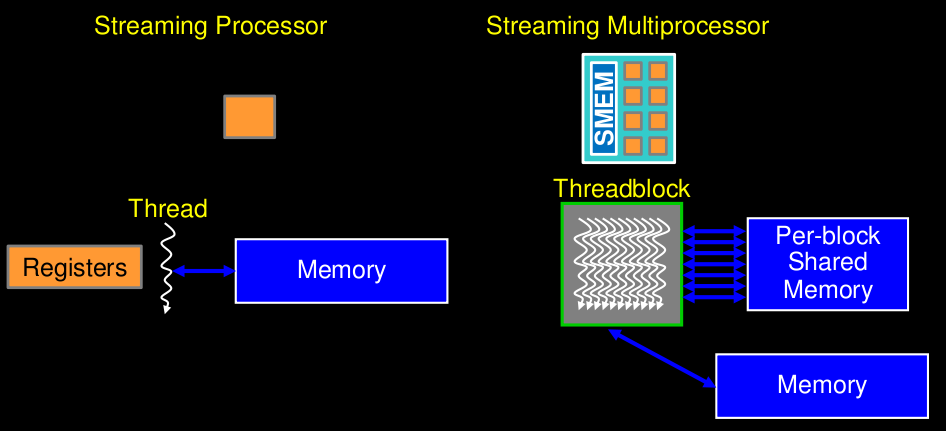
\includegraphics[scale=0.5]{images/S-6.png}
\end{center}
\end{frame}
%% ============================================================================
%% ============================================================================
\begin{frame}[fragile]
\frametitle{Hardware multithreading}

\begin{itemize}
\item \textcolor{blue}{\bf Hardware allocates resources to blocks}:
\begin{itemize}
\item blocks need: thread slots, registers, shared memory
\item blocks don't run until resources are available
\end{itemize}
\item \textcolor{blue}{\bf Hardware schedules threads}:
\begin{itemize}
\item hreads have their own registers
\item any thread not waiting for something can run
\item context switching is free – every cycle
\end{itemize}
\item \textcolor{blue}{\bf Hardware relies on threads to hide latency}:
\begin{itemize}
\item thus high  parallelism is necessary for performance.
\end{itemize}
\end{itemize}


\begin{center}
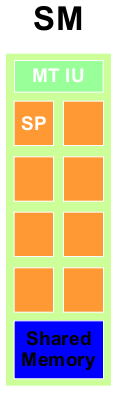
\includegraphics[scale=0.35]{images/39.png}
\end{center}
\end{frame}
%% ============================================================================
%% ============================================================================
\begin{frame}[fragile]
\frametitle{SIMT thread execution}

\begin{itemize}
\item  At each clock cycle, a   
      multiprocessor executes the same
     instruction on a group of threads
     called a \textcolor{blue}{\bf warp}
\begin{itemize}
\item  The number of threads in a warp is
      the \textcolor{blue}{\bf warp size} (32 on G80)
\item A half-warp is the first or second
      half of a warp.
\end{itemize}
%%
\item  Within a warp, threads
\begin{itemize}
%% \item always executing same instruction
\item  share instruction fetch/dispatch
\item  some become inactive when code path diverges
\item  hardware automatically handles divergence
\end{itemize}
%%
\item   \textcolor{blue}{\bf  Warps are the primitive unit of scheduling}:
\begin{itemize}
\item each active block is split nto warps in a well-defined way
\item threads within a warp are executed physically in
      parallel while warps and blocks are executed logically in
      parallel.
\end{itemize}
\end{itemize}

\begin{center}
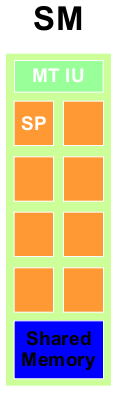
\includegraphics[scale=0.25]{images/39.png}
\end{center}
\end{frame}
%% ============================================================================
